\documentclass{article}

\usepackage{amsmath}
\usepackage{amssymb}
\usepackage{tikz}
\usepackage{pgfplots}

\begin{document}
	
\author{Logan Grosz}
\title{Inverse Trigonometric Function Derivatives}
\date{\today}

\maketitle

\begin{abstract}
	\noindent The derivatives of inverse trigonometric derivatives are very different than their basic trigonometric counterparts. The following document will describe the process of getting such a visually unorthodox solution to $\frac{d}{dx}\,f$, where $f$ is an inverse trigonometric function.
\end{abstract}

\section{Declarations}
	$x$; parameter passed into inverse trigonometric function, measured in radians;\\
	\indent$\text{For} \,\,\sin^{-1} x, x \in [-1,1]$\\
	\indent$\text{For} \,\,\cos^{-1} x, x \in [-1,1]$\\
	\indent$\text{For} \,\,\tan^{-1} x, x \in [-\infty,\infty]$\\
	\indent$\text{For} \,\,\cot^{-1} x, x \in [-\infty,\infty]$\\
	\indent$\text{For} \,\,\sec^{-1} x, x \in (-\infty,-1]\cup[1,\infty)$\\
	\indent$\text{For} \,\,\csc^{-1} x, x \in (-\infty,-1]\cup[1,\infty)$\\
	$\theta \triangleq x$; used in place of x at times to not confused reader;\\
	$\text{arc}f \triangleq f^{-1}$; arc and -1 convention equivalence; $\arcsin x \equiv \sin^{-1}x$\\
	$hypotenuse$;Latin for "stretching under", the line connecting both catheti; $\text{Short: }hyp$\\
	$adjacent$; Cathetus closest or next to the observed angle; $\text{Short: }adj$\\
	$opposite$ Cathetus furthest from or opposite of the observed angle;$\text{Short: }opp$
\section{Rule}

\begin{align}
	\dfrac{d}{dx}\sin^{-1}\,x&=\dfrac{1}{\sqrt{1 - x^2}}\\[1em]
	\dfrac{d}{dx}\cos^{-1}\,x&=\dfrac{-1}{\sqrt{1 - x^2}}\\[1em]
	\dfrac{d}{dx}\tan^{-1}\,x&=\dfrac{1}{x^2+1}\\[1em]
	\dfrac{d}{dx}\cot^{-1}\,x&=\dfrac{-1}{x^2+1}\\[1em]
	\dfrac{d}{dx}\sec^{-1}\,x&=\dfrac{1}{|x|\sqrt{x^2-1}}\\[1em]
	\dfrac{d}{dx}\csc^{-1}\,x&=\dfrac{-1}{|x|\sqrt{x^2-1}}
\end{align}

\section{Pre-Derivation}
\noindent The following notation is the inverse of its subscribed function:
$$\sin^{-1}(\sin \theta)=\theta$$

\noindent Pythagorean Trigonometric Identity:
$$sin^2\theta+cos^2\theta=1$$

\noindent The following defines sides of triangle given angle measure $\theta$.
\begin{center}
	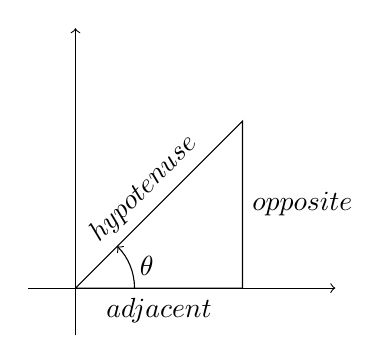
\begin{tikzpicture}[scale = 3]
	\draw[->] (0,-0.2) -- (0, 1.1);
	\draw[->] (-0.2,0) -- (1.1,0);
	\draw (0,0) -- node[sloped,above]{$hypotenuse$} (0.707107,0.707107) -- node[anchor = west]{$opposite$} (0.707107,0) -- node[sloped,below]{$adjacent$} (0,0);
	\draw[->] (0.25,0) arc (0:45:0.25) node [midway, right] {$\theta$};
	\end{tikzpicture}
\end{center}

%All trig functions, some had to be expaned so pgfplots would plot them
\newpage
\noindent The following are the graphs of all six inverse trigonometric functions for reference:\\
\begin{tabular}{c c}
	$y=sin^{-1}x$ & $y=cos^{-1}x$\\
	\parbox[c]{0.5\textwidth}{
	\begin{tikzpicture}[scale = 0.75]
		\begin{axis}[
			trig format plots=rad,
			samples=300,
			axis lines=middle,enlargelimits=true,
		]
		\addplot[
			no markers,
			blue,
			thick,
			domain=-1:1
		] {asin(x)};
		\end{axis}
	\end{tikzpicture}}
	&
	\parbox[c]{0.5\textwidth}{
	\begin{tikzpicture}[scale=0.75]
		\begin{axis}[
			trig format plots=rad,
			samples=300,
			axis lines=middle,enlargelimits=true,
		]
		\addplot[
			no markers,
			blue,
			thick,
			domain=-1:1
		] {acos(x)};
		\end{axis}
	\end{tikzpicture}}\\
	\rule{0pt}{6ex}
	$y=tan^{-1}x$ & $y=cot^{-1}x$\\
	\parbox[c]{0.5\textwidth}{
		\begin{tikzpicture}[scale=0.75]
			\begin{axis}[
				trig format plots=rad,
				samples=300,
				axis lines=middle,enlargelimits=true,
			]
			\addplot[
				no markers,
				blue,
				thick,
				domain=-4:4
			] {atan(x)};
			\end{axis}
		\end{tikzpicture}}
	&
	\parbox[c]{0.5\textwidth}{
		\begin{tikzpicture}[scale=0.75]
			\begin{axis}[
				trig format plots=rad,
				samples=300,
				axis lines=middle,enlargelimits=true,
			]
			\addplot[
				no markers,
				blue,
				thick,
				domain=-4:4
			] {pi - atan(x)};
			\end{axis}
		\end{tikzpicture}}\\
	\rule{0pt}{6ex}
	$y=sec^{-1}x$ & $y=csc^{-1}x$\\
	\parbox[c]{0.5\textwidth}{
		\begin{tikzpicture}[scale=0.75]
			\begin{axis}[
				trig format plots=rad,
				samples=300,
				axis lines=middle,enlargelimits=true,
			]
			\addplot[
				no markers,
				blue,
				thick,
				domain=-10:-1
			] {acos(1/x)};
			\addplot[
				no markers,
				blue,
				thick,
				domain=1:10
			] {acos(1/x)};
			\end{axis}
		\end{tikzpicture}}
		&
		\parbox[c]{0.5\textwidth}{
		\begin{tikzpicture}[scale=0.75]
			\begin{axis}[
				trig format plots=rad,
				samples=300,
				axis lines=middle,enlargelimits=true,
			]
			\addplot[
				no markers,
				blue,
				thick,
				domain=-10:-1
			] {asin(1/x)};
			\addplot[
				no markers,
				blue,
				thick,
				domain=1:10
			] {asin(1/x)};
			\end{axis}
		\end{tikzpicture}}\\
\end{tabular}
\newpage

\section{Derivation}

\subsection{Inverse Sine}
	\begin{gather*}
		y = \sin^{-1} x\\
		\sin y = x\\
		\dfrac{d}{dx} \sin y = \dfrac{d}{dx} x\\
		\dfrac{dy}{dx} \cos y = 1\\
		\dfrac{dy}{dx} = \dfrac{1}{\cos y}\\
		\\
		\text{Using $\sin^2y+cos^2y=1$...}\\
		\cos y = \sqrt{1-\sin^2y}\\
		\\
		\dfrac{dy}{dx} = \dfrac{1}{\sqrt{1-sin^2y}}\\
		\\
		\text{Recall $\sin y = x$...}\\
		\therefore \dfrac{d}{dx}\sin^{-1}x = \dfrac{1}{\sqrt{1-x^2}}
	\end{gather*}

Id Est\\
%\parbox or \multicolumn can be used to align tikz pictures and text in center vertically
	\begin{tabular}{c c}
		\parbox[c]{0.5\textwidth}{
			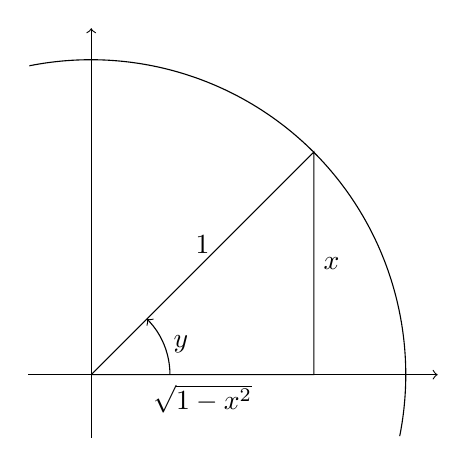
\begin{tikzpicture}[scale = 4]
				%axis and arc
				\draw[->] (0,-0.2) -- (0, 1.1);
				\draw[->] (-0.2,0) --(1.1,0);
				\draw (-0.19635,0.980785) arc (101.25:-11.25:1);
				%reference triangle
				\draw (0,0) -- node[midway, above]{$1$} (0.707107,0.707107) -- node[midway, right]{$x$} (0.707107,0) -- node[midway, below]{$\sqrt{1-x^2}$} (0,0);
				%degree measure 'y'
				\draw[->] (0.25,0) arc (0:45:0.25) node [midway, right] {$y$};
			\end{tikzpicture}}
			&
		\parbox[c]{0.5\textwidth}{
				\begin{gather*}
				\sin y = x\Rightarrow\dfrac{opp}{hyp} = \dfrac{x}{1}\\
				\\
				\text{See above that...}\\
				\dfrac{dy}{dx}=\dfrac{1}{\cos x}\\
				\\
				\text{See figure at left...}\\
				\cos y = \sqrt{1-x^2}\\
				\\
				\therefore \dfrac{d}{dx}\sin^{-1}x=\dfrac{1}{\sqrt{1-x^2}}
				\end{gather*}}
	\end{tabular}

\subsection{Inverse Cosine}
	\begin{gather*}
		y = \cos^{-1} x\\
		\cos y = x\\
		\dfrac{d}{dx} \cos y = \dfrac{d}{dx} x\\
		\dfrac{dy}{dx} -\sin y = 1\\
		\dfrac{dy}{dx} = \dfrac{-1}{\sin y}\\
		\\
		\text{Using $\sin^2y+cos^2y=1$...}\\
		\sin y = \sqrt{1-\cos^2 y}\\
		\\
		\dfrac{dy}{dx} = \dfrac{-1}{\sqrt{1-cos^2y}}\\
		\\
		\text{Recall $\cos y = x$...}\\
		\therefore \dfrac{d}{dx}\cos^{-1}x = \dfrac{-1}{\sqrt{1-x^2}}
	\end{gather*}

Id Est\\
	\begin{tabular}{c c}
		\parbox[c]{0.5\textwidth}{
			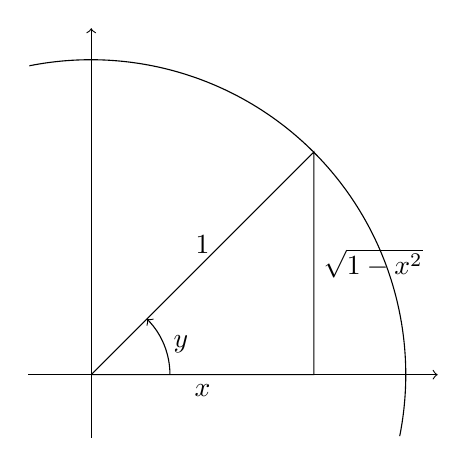
\begin{tikzpicture}[scale = 4]
				%axis and arc
				\draw[->] (0,-0.2) -- (0, 1.1);
				\draw[->] (-0.2,0) --(1.1,0);
				\draw (-0.19635,0.980785) arc (101.25:-11.25:1);
				%reference triangle
				\draw (0,0) -- node[midway, above]{$1$} (0.707107,0.707107) -- node[midway, right]{$\sqrt{1-x^2}$} (0.707107,0) -- node[midway, below]{$x$} (0,0);
				%degree measure 'y'
				\draw[->] (0.25,0) arc (0:45:0.25) node [midway, right] {$y$};
			\end{tikzpicture}}
		&
		\parbox[c]{0.5\textwidth}{
			\begin{gather*}
			\cos y = x\Rightarrow\dfrac{adj}{hyp} = \dfrac{x}{1}\\
			\\
			\text{See above that...}\\
			\dfrac{dy}{dx}=\dfrac{-1}{\sin y}\\
			\\
			\text{See figure at left...}\\
			\sin y = \sqrt{1-x^2}\\
			\\
			\therefore \dfrac{d}{dx}\cos^{-1}x=\dfrac{-1}{\sqrt{1-x^2}}
			\end{gather*}}
	\end{tabular}

\subsection{Inverse Tangent}
\begin{gather*}
	y = \tan^{-1} x\\
	\tan y = x\\
	\dfrac{d}{dx} \tan y = \dfrac{d}{dx} x\\
	\dfrac{dy}{dx} \sec^2 y = 1\\
	\dfrac{dy}{dx} = \dfrac{1}{\sec^2 y}\\
	\\
	\text{Using $\sin^2y+cos^2y=1$...}\\
	\sec^2 y = \tan^2 y + 1\\
	\dfrac{dy}{dx} = \dfrac{1}{\tan^2 y + 1}\\
	\\
	\text{Recall $\tan y = x$...}\\
	\therefore \dfrac{d}{dx}\tan^{-1}x = \dfrac{1}{x^2 + 1}
\end{gather*}

Id Est\\
\begin{tabular}{c c}
	\parbox[c]{0.5\textwidth}{
		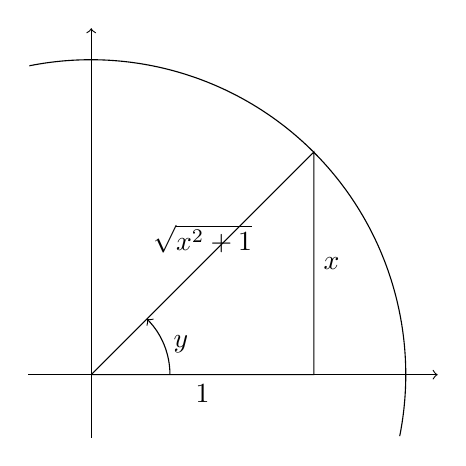
\begin{tikzpicture}[scale = 4]
			%axis and arc
			\draw[->] (0,-0.2) -- (0, 1.1);
			\draw[->] (-0.2,0) --(1.1,0);
			\draw (-0.19635,0.980785) arc (101.25:-11.25:1);
			%reference triangle
			\draw (0,0) -- node[midway, above]{$\sqrt{x^2 + 1}$} (0.707107,0.707107) -- node[midway, right]{$x$} (0.707107,0) -- node[midway, below]{$1$} (0,0);
			%degree measure 'y'
			\draw[->] (0.25,0) arc (0:45:0.25) node [midway, right] {$y$};
		\end{tikzpicture}}
	&
	\parbox[c]{0.5\textwidth}{
		\begin{gather*}
			\tan y = x\Rightarrow\dfrac{opp}{adj} = \dfrac{x}{1}\\
			\\
			\text{See above that...}\\
			\dfrac{dy}{dx}=\dfrac{1}{\sec^2 y}\\
			\\
			\text{See figure at left...}\\
			\sec^2 y = x^2 + 1\\
			\\
			\therefore \dfrac{d}{dx}\tan^{-1}x=\dfrac{1}{x^2 + 1}
		\end{gather*}}
\end{tabular}
	
\subsection{Inverse Cotangent}
\begin{gather*}
	y = \cot^{-1} x\\
	\cot y = x\\
	\dfrac{d}{dx} \cot y = \dfrac{d}{dx} x\\
	\dfrac{dy}{dx} -\csc^2 y = 1\\
	\dfrac{dy}{dx} = \dfrac{-1}{\csc^2 y}\\
	\\
	\text{Using $\sin^2y+cos^2y=1$...}\\
	\csc^2 y = \cot^2 y + 1\\
	\dfrac{dy}{dx} = \dfrac{-1}{\cot^2 y + 1}\\
	\\
	\text{Recall $\cot y = x$...}\\
	\therefore \dfrac{d}{dx}\cot^{-1}x = \dfrac{-1}{x^2 + 1}
\end{gather*}

Id Est\\
\begin{tabular}{c c}
	\parbox[c]{0.5\textwidth}{
		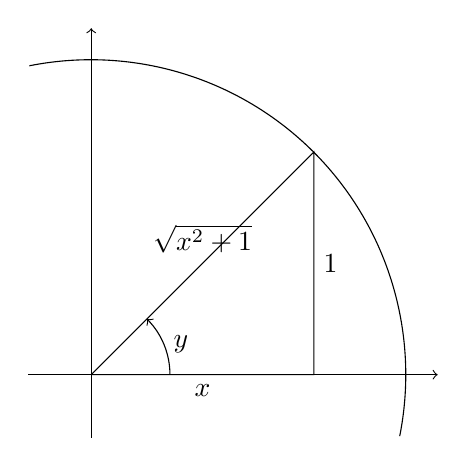
\begin{tikzpicture}[scale = 4]
			%axis and arc
			\draw[->] (0,-0.2) -- (0, 1.1);
			\draw[->] (-0.2,0) --(1.1,0);
			\draw (-0.19635,0.980785) arc (101.25:-11.25:1);
			%reference triangle
			\draw (0,0) -- node[midway, above]{$\sqrt{x^2 + 1}$} (0.707107,0.707107) -- node[midway, right]{$1$} (0.707107,0) -- node[midway, below]{$x$} (0,0);
			%degree measure 'y'
			\draw[->] (0.25,0) arc (0:45:0.25) node [midway, right] {$y$};
		\end{tikzpicture}}
	&
	\parbox[c]{0.5\textwidth}{
		\begin{gather*}
			\cot y = x\Rightarrow\dfrac{adj}{opp} = \dfrac{x}{1}\\
			\\
			\text{See above that...}\\
			\dfrac{dy}{dx}=\dfrac{-1}{\csc^2 y}\\
			\\
			\text{See figure at left...}\\
			\csc^2 y = x^2 + 1\\
			\\
			\therefore \dfrac{d}{dx}\cot^{-1}x=\dfrac{-1}{x^2 + 1}
		\end{gather*}}
\end{tabular}

%I could'nt find a purely algebraic derivation of this formula
\subsection{Inverse Secant}
\begin{gather*}
	y = \sec^{-1} x\\
	\sec y = x\\
	\dfrac{d}{dx} \sec y = \dfrac{d}{dx} x\\
	\dfrac{dy}{dx} \sec y \tan y = 1\\
	\dfrac{dy}{dx} = \dfrac{1}{\sec y \tan y}\\
	\\
\end{gather*}

Id Est\\
\begin{tabular}{c c}
	\parbox[c]{0.5\textwidth}{
		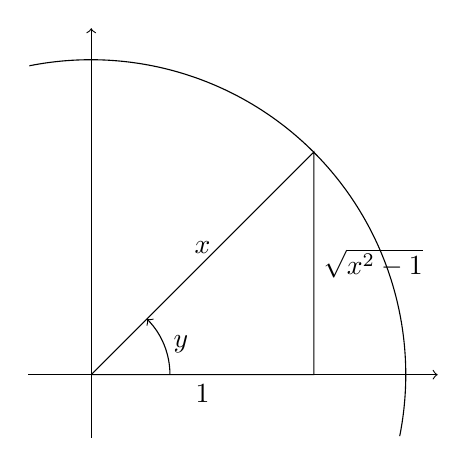
\begin{tikzpicture}[scale = 4]
			%axis and arc
			\draw[->] (0,-0.2) -- (0, 1.1);
			\draw[->] (-0.2,0) --(1.1,0);
			\draw (-0.19635,0.980785) arc (101.25:-11.25:1);
			%reference triangle
			\draw (0,0) -- node[midway, above]{$x$} (0.707107,0.707107) -- node[midway, right]{$\sqrt{x^2 - 1}$} (0.707107,0) -- node[midway, below]{$1$} (0,0);
			%degree measure 'y'
			\draw[->] (0.25,0) arc (0:45:0.25) node [midway, right] {$y$};
		\end{tikzpicture}}
	&
	\parbox[c]{0.5\textwidth}{
		\begin{gather*}
			\sec y = x\Rightarrow\dfrac{hyp}{adj} = \dfrac{x}{1}\\
			\\
			\text{See above that...}\\
			\dfrac{dy}{dx}=\dfrac{1}{\sec y \tan y}\\
			\\
			\text{See figure at left...}\\
			\tan y = \sqrt{x^2 + 1}\\
			\\
			\text{Recall $\sec y = x$}\\
			\text{And note $\dfrac{d}{dx}\sec^{-1}\theta > 0$, so, $|x|= \{x| x > 0\}$}\\
			\therefore \dfrac{d}{dx}\sec^{-1}x=\dfrac{1}{|x|\sqrt{x^2 - 1}}
		\end{gather*}}
\end{tabular}

%I could'nt find a purely algebraic derivation of this formula
\subsection{Inverse Cosecant}
\begin{gather*}
	y = \csc^{-1} x\\
	\csc y = x\\
	\dfrac{d}{dx} \csc y = \dfrac{d}{dx} x\\
	\dfrac{dy}{dx} -\csc y \cot y = 1\\
	\dfrac{dy}{dx} = \dfrac{1}{\csc y \cot y}\\
	\\
\end{gather*}

Id Est\\
\begin{tabular}{c c}
	\parbox[c]{0.5\textwidth}{
		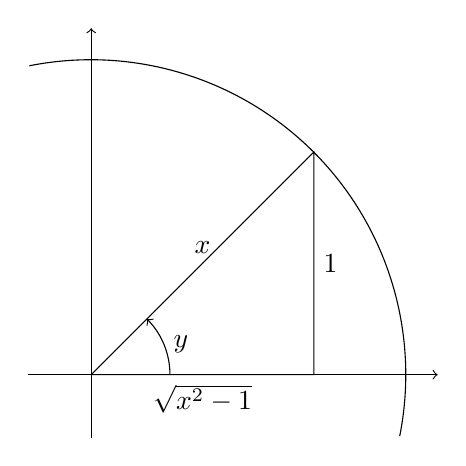
\begin{tikzpicture}[scale = 4]
			%axis and arc
			\draw[->] (0,-0.2) -- (0, 1.1);
			\draw[->] (-0.2,0) --(1.1,0);
			\draw (-0.19635,0.980785) arc (101.25:-11.25:1);
			%reference triangle
			\draw (0,0) -- node[midway, above]{$x$} (0.707107,0.707107) -- node[midway, right]{$1$} (0.707107,0) -- node[midway, below]{$\sqrt{x^2 - 1}$} (0,0);
			%degree measure 'y'
			\draw[->] (0.25,0) arc (0:45:0.25) node [midway, right] {$y$};
		\end{tikzpicture}}
	&
	\parbox[c]{0.5\textwidth}{
		\begin{gather*}
			\csc y = x\Rightarrow\dfrac{hyp}{opp} = \dfrac{x}{1}\\
			\\
			\text{See above that...}\\
			\dfrac{dy}{dx}=\dfrac{-1}{\csc y \cot y}\\
			\\
			\text{See figure at left...}\\
			\cot y = \sqrt{x^2 + 1}\\
			\\
			\text{Recall $\csc y = x$}\\
			\text{And note, $\dfrac{d}{dx}\csc^{-1}\theta < 0$, so, $|x|= \{x| x > 0\}$}\\
			\therefore \dfrac{d}{dx}\csc^{-1}x=\dfrac{-1}{|x|\sqrt{x^2 - 1}}
		\end{gather*}}
\end{tabular}

%Have not been added yet
\section{Exempli Gratia}

Examples of important instances

\end{document}